\documentclass[11pt]{article}
%\renewcommand\refname{ }

\usepackage{fullpage}
\usepackage{epsfig}
\usepackage{graphicx}
\usepackage{listings,color}
\usepackage[dvipsnames]{xcolor}
\usepackage{tcolorbox}
\usepackage{natbib}
\usepackage{subfig}

\input macros.tex

\begin{document}

\begin{center} 
\bfseries{
\begin{large}
  Response to referee report for manuscript ref. MN-23-2721-MJ
\end{large}
}
\end{center}

\begin{tcolorbox}[colback={lightgray}]
    The authors focus on the impacts of the neutron star merger (NSM) on the formation of second-generation stars in first galaxies. Following r-process elements with cosmological simulations is unique and interesting. However, important information about the modeling NSM is lacking in the current manuscript. Also, consideration of the simulation results is not enough. I hope the authors revise the manuscript based on the following comments.
\end{tcolorbox}

We thank the referee for their review of our work, and we have
addressed their points individually below.  In the manuscript, we have
boldfaced the added text and crossed out the deleted text.  

\begin{tcolorbox}[colback={lightgray}]
    1)      The authors assume that neutron star binaries merge after 10, 30, or 100 Myr. These time scales are too short (Belczynski et al. 2002, ApJ, 572, 407; Kinugawa et al. 2014, MNRAS, 442, 2963). What kind of binary parameters did you assume? Is it reasonable? Without reasonable explanations about the short merger timescales, I cannot believe that NSMs happened in the early Universe.
\end{tcolorbox}

We agree that the time scales we have explored are very short, but we are exploring a very particular scenario, and the delay times that we have chosen are not yet out of the realm of possibilities. \citet{Hirai15} quote the lower limit of a delay time to be $\sim10$ Myr, and that delay times of $\sim100$ Myr can explain the scatter in [Eu/Fe] for metal-poor stars in the galactic halo. 

\citet{Frebel23} also summarize the current state of discussion around the merger times for NSMs. They quote the minimum delay time to be between 10--100 Myr based on work done by other authors, and that there is some discussion that even shorter delay times of about 1 Myr could be possible.

For Reticulum II (Ret II) in particular, a long delay time of a couple Gyr is not compatible with the r-process enhanced stars. \citet{Simon23} provide an explanation for the timing requirements for r-process enrichment in Ret II, and they find that a NSM must occur within 500 Myr in order to reproduce the abundances and allow for thorough mixing. This requires the NSM to occur well before the formation of second generation stars.

Enzo does not have the capability to follow binary system formation. We simply do not have the resolution to accomplish such a task in a cosmological setting. Because of this, our NSM model is an extremely ideal scenario, where we do not have to pick binary system parameters. The question of how this binary system formed in the first place is outside of the scope of this paper and would require significant modifications to the code base in order for that to happen in our simulations. We are assuming that there could exist a possibility where this type of binary system could form and then go on to merge together. Based on work cited above, we are comfortable with the delay times we have chosen, and they could add further information about the possibility of these short time delays moving forward.

We are certainly simulating a particular scenario. We are operating under the assumption that if a NSM did occur in a galaxy like Ret II, then it would have to happen fairly early in order to allow for enough time to pass for thorough mixing to take place. We would also like to remind the referee that this is a ``proof-of-concept'' test of our model to investigate how the NSM may affect the second generation of stars. We are not trying to exactly reproduce Ret II, but we want to begin to understand what are the effects of a NSM of this type early in the history of a galaxy. We would like to let the referee know that there is a follow up plan to this simulation, with more papers to come.

\textbf{(DS to-do)} We have added this explanation to SECTION.

\textbf{DS Notes:}

https://arxiv.org/pdf/2212.00810.pdf
\begin{itemize}
    \item for reticulum II, longer delay times (~couple Gyr) are incompatible with r-process stars in Ret II
    \item must merge within about 500 Myr for Ret II
    \item there is uniformity among the r-process enriched stars, indicating that thorough mixing needs to take place before star formation can occur. To allow for enough time, the NSM has to happen relatively early in the star formation history of ret II
\end{itemize}

https://arxiv.org/pdf/2302.09188.pdf
\begin{itemize}
    \item minimum delay time of 10-100 Myr
    \item there is some argument that merging could happen on the order of 1 Myr
    \item still lots of debate around the specifics
\end{itemize}


\begin{tcolorbox}[colback={lightgray}]
    2)      NS binaries can form even in Population I/II stars, particularly in dense star clusters. Why do you consider NS binaries originated from Population III stars. The binary fraction and ISM of population III stars are still under debate. The authors should describe the motivation of NSM originating from population III stars.
\end{tcolorbox}

The motivation of this work came from the results of the r-process enhanced stars in Ret II. For these stars, a NSM occurring early in the star formation history of the galaxy can explain the enhancement. We were interested in the possibility of the NSM occurring early enough in the history of the galaxy to be a descendant of Pop III stars. We ask this question near the end of the Introduction: ``... what happens if a single NSM, produced from the remnants of Pop III stars, occurs within a galaxy in the early universe?'' This is the question that we are exploring in this work.

We do not consider any binary system formation for Pop II stars in this work to isolate the effects from a NSM from a Pop III system alone. We are thus only considering the binary system formation, and subsequent merging, of the NSs. This would be an interesting thing to explore in the future however.

\textbf{(DS to-do)} We have made our motivation more clear in SECTION.

\begin{tcolorbox}[colback={lightgray}]
    3)      The current abstract consists of a general introduction and expectable trends. The authors should rewrite the text of the abstract significantly with solid conclusions and values taken from the detailed simulations.
\end{tcolorbox}

\textbf{DS Notes:}
Replace two general sentences with these more specific ones.
\begin{itemize}
    \item A high explosion energy leads to a Pop II mass fraction of 72\% being highly enhanced with r-process elements, while a lower explosion energy leads to a Pop II mass fraction of 80\% being r-process enhanced, but only 14\% being highly enhanced.
    \item When the NSM has a short delay time of 10 Myr, only 5\% of the mass fraction of Pop II stars is highly r-process enhanced, while 64\% of the mass fraction of Pop II stars is highly r-process enhanced for the longest delay time of 100 Myr. 
\end{itemize}

\begin{tcolorbox}[colback={lightgray}]
    4)      It looks like one of the main points of the manuscript is revealing the impacts of NSM on the physical properties of the first galaxies with Pop II star formation. An NSM is an additional feedback source at the point of the first galaxy formation. I think the impact of NSM is degenerated with other factors of Pop III stars like the number of stars in mini-haloes, star formation efficiency, and initial mass function. For example, if three Pop III stars form in mini-halos (e.g., Sugimura et al. 2020, ApJ, 892, L14; Sugimura et al. 2023), they are likely to give similar feedback. The authors should add a discussion about the uniqueness of NSMs at the point of the first galaxy formation.
\end{tcolorbox}

\textbf{DS Notes:}
\begin{itemize}
    \item I feel like the main thing that makes NSM unique is their production of r-process elements (along with the effects of a kilonova, but maybe we don't mention that?). One of the main points is that NSMs can produce r-process enhanced stars, but also that the exact feedback mechanisms that occur appear to drastically affect results (last bullet point in conclusions). So we cannot pick apart the impacts of NSM on the physical properties of the first galaxies with Pop II star formation -- this was not something that we were trying to address really at all?
    \item \jhw{I agree that the primary focus is the r-process enhancement and not the energetics.  This is especially true because they will happen later in the halo's evolution when the mass is greater and potential is deeper, making its effect lesser than Pop III feedback and then Pop II feedback that has a large effect primarily due to the larger amount of stars that form.  You can take the Pop III stellar masses from our 2020 paper and estimate the amount of energy released in radiation and SNe and show that it's much greater than a kilonova.  This would be a useful comparison to add to the discussion.}
\end{itemize}

\begin{tcolorbox}[colback={lightgray}] 
    5)      Considerations about the simulation results are not enough. For example, in Sec. 3.2, the authors say, “The Pop II stellar mass follows a relatively similar trend in each run, but the NSM runs end with larger Pop II stellar masses as compared to the original run.” Why do NSMs induce the larger Pop II stellar masses? Please describe the physical reasons because it is complicated due to a combination of more metal enrichment and gas blowout.
\end{tcolorbox}

\textbf{DS Notes:}
\begin{itemize}
    \item Yes, this is a good question and one that I thought we made pretty clear. The answer to this is ``I don't know''. There are a lot of details to pick through in these simulations, and making comparisons across the simulations is a complicated task. Because we don't have a large sample size to study, it's hard to say anything conclusive about how the NSM might affect the Pop II stellar masses, and whether other star formation and feedback is affecting it as well. This is a question we are continuing to explore. In this paper, we are simply reporting on the results.
    \item \jhw{Yes, we should tell the referee that the causes of these diffenences are difficult to determine and that we will defer to a deeper study to a later paper because this paper primarily focuses on the enrichment.}
    \item We did find that NSM runs have higher cold gas mass fractions at late times. This could be one possible explanation for this.
\end{itemize}

\begin{tcolorbox}[colback={lightgray}]
    Minor comments:
    6)      Is Sec. 3.1. about the original (without NSM) run? It would be better to write it.
\end{tcolorbox}

Yes, Sec. 3.1 is about the original run. We have changed this section title and added a bit of text to reflect that.

\begin{tcolorbox}[colback={lightgray}]
    7)      Figure 6 shows “P3 metallicity fraction”. What is the P3 metallicity?
\end{tcolorbox}

We apologize for this, the caption was correct, but the label in the plot was wrong. The label should have read ``Total Metallicity Fraction'' instead of ``P3 Metallicity Fraction''. The total metallicity is the metallicity of the stars from both Pop II and Pop III sources. We have fixed this plot.

\begin{tcolorbox}[colback={lightgray}]
    8)      Purple lines in Figures 3, 5, and 8 show “Hyp.”. What is the meaning of Hyp.?
\end{tcolorbox}

We apologize for that confusion. ``Hyp.'' stood for ``hypernova'' which is how the original Pop III star ends its life. To keep things simple, we have changed that in the plots to say ``OG'' to make it clear that those lines correspond to the original run with no NSM.  \jhw{Did you refer to the OG simulation as the original run in the caption?  We should explicitly state this for non-native speakers and boomers.}

\begin{tcolorbox}[colback={lightgray}]
    9)      The authors show the coexistence of Pop II and III stars in the first galaxies. Recent theoretical studies showed similar results (Riaz et al. 2022, ApJL, 937, L6; Yajima et al., arXiv2211.12970). It would be good to discuss the mass fraction and distribution of Pop III stars in the first galaxies with the previous works. 
\end{tcolorbox}

\textbf{DS Notes:}
\begin{figure}[h]
    \centering
    \subfloat[\centering Energy Variation]{{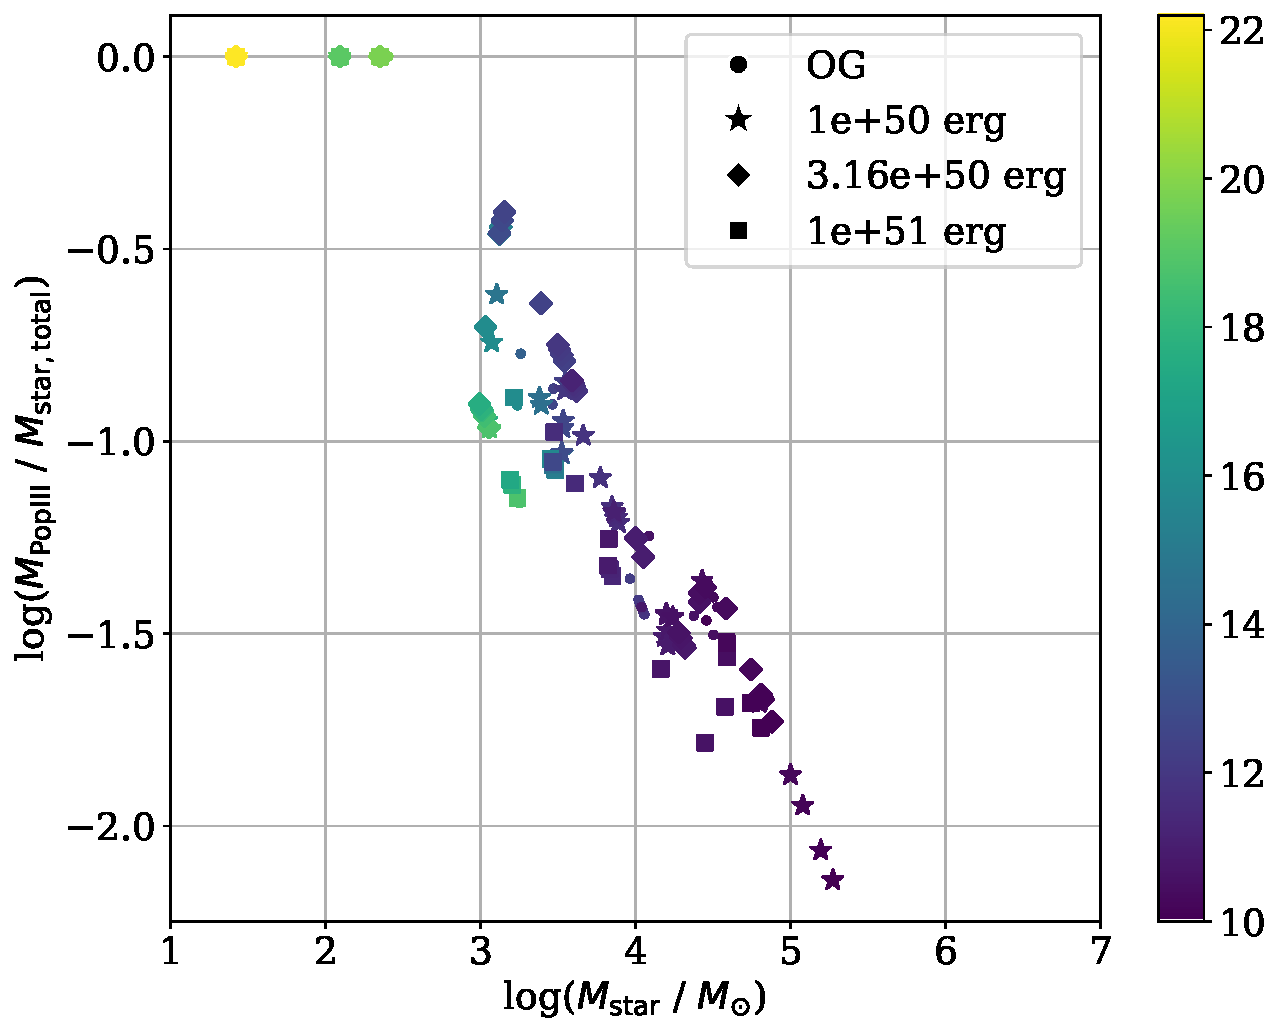
\includegraphics[width=0.4\textwidth]{plots/eng_pop3_ratio.pdf} }}%
    \qquad
    \subfloat[\centering Delay Time Variation]{{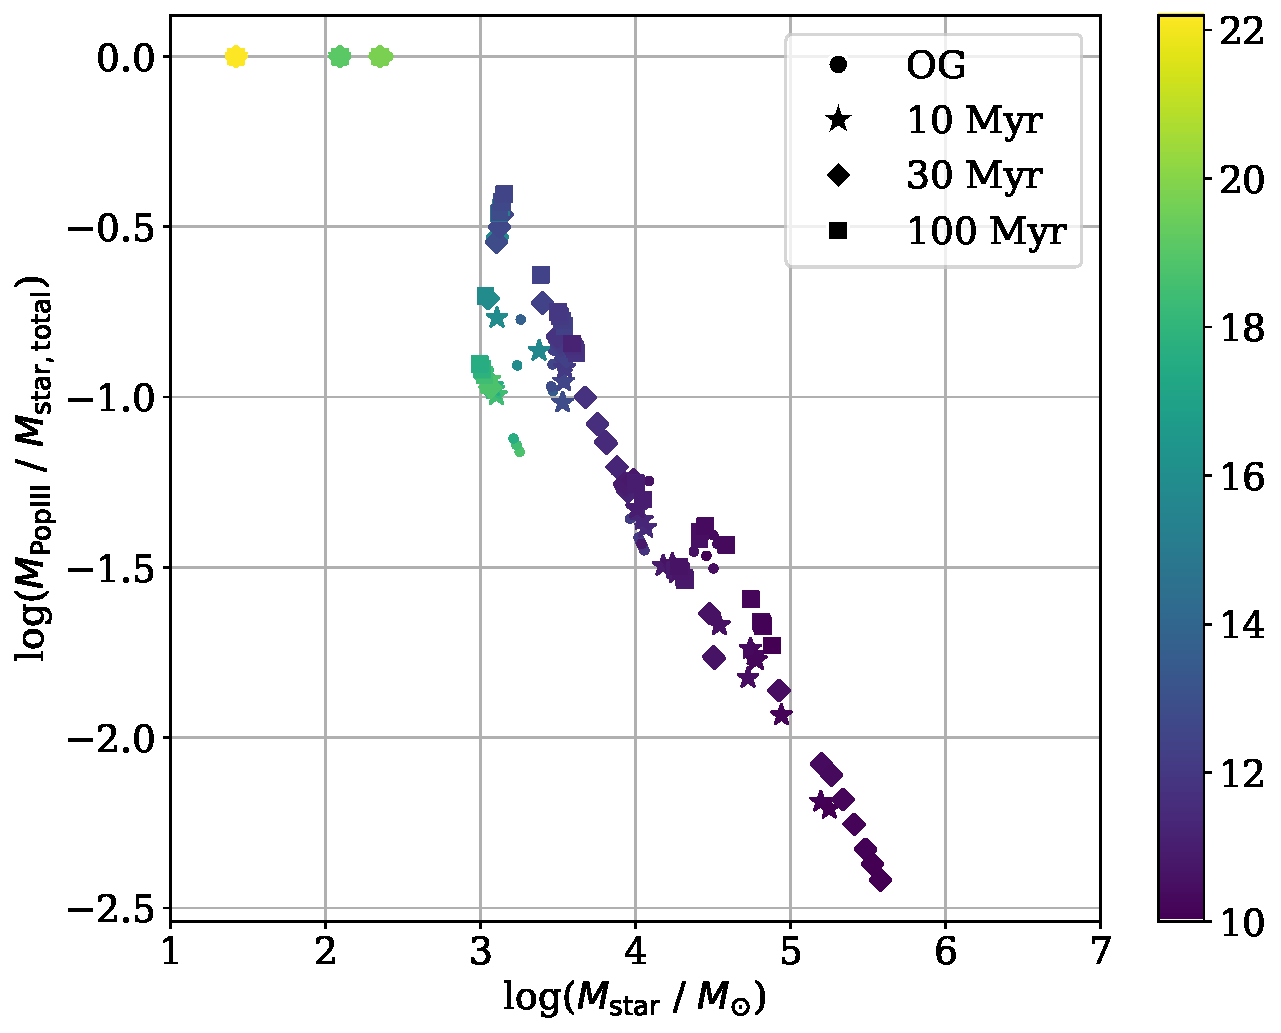
\includegraphics[width=0.4\textwidth]{plots/time_pop3_ratio.pdf} }}%
    \caption{The mass fraction of Pop III stars to total stellar mass versus the total stellar mass colored by redshift.}%
    \label{fig:ratio}%
\end{figure}

\begin{figure}[h]
    \centering
    \subfloat[\centering Energy Variation]{{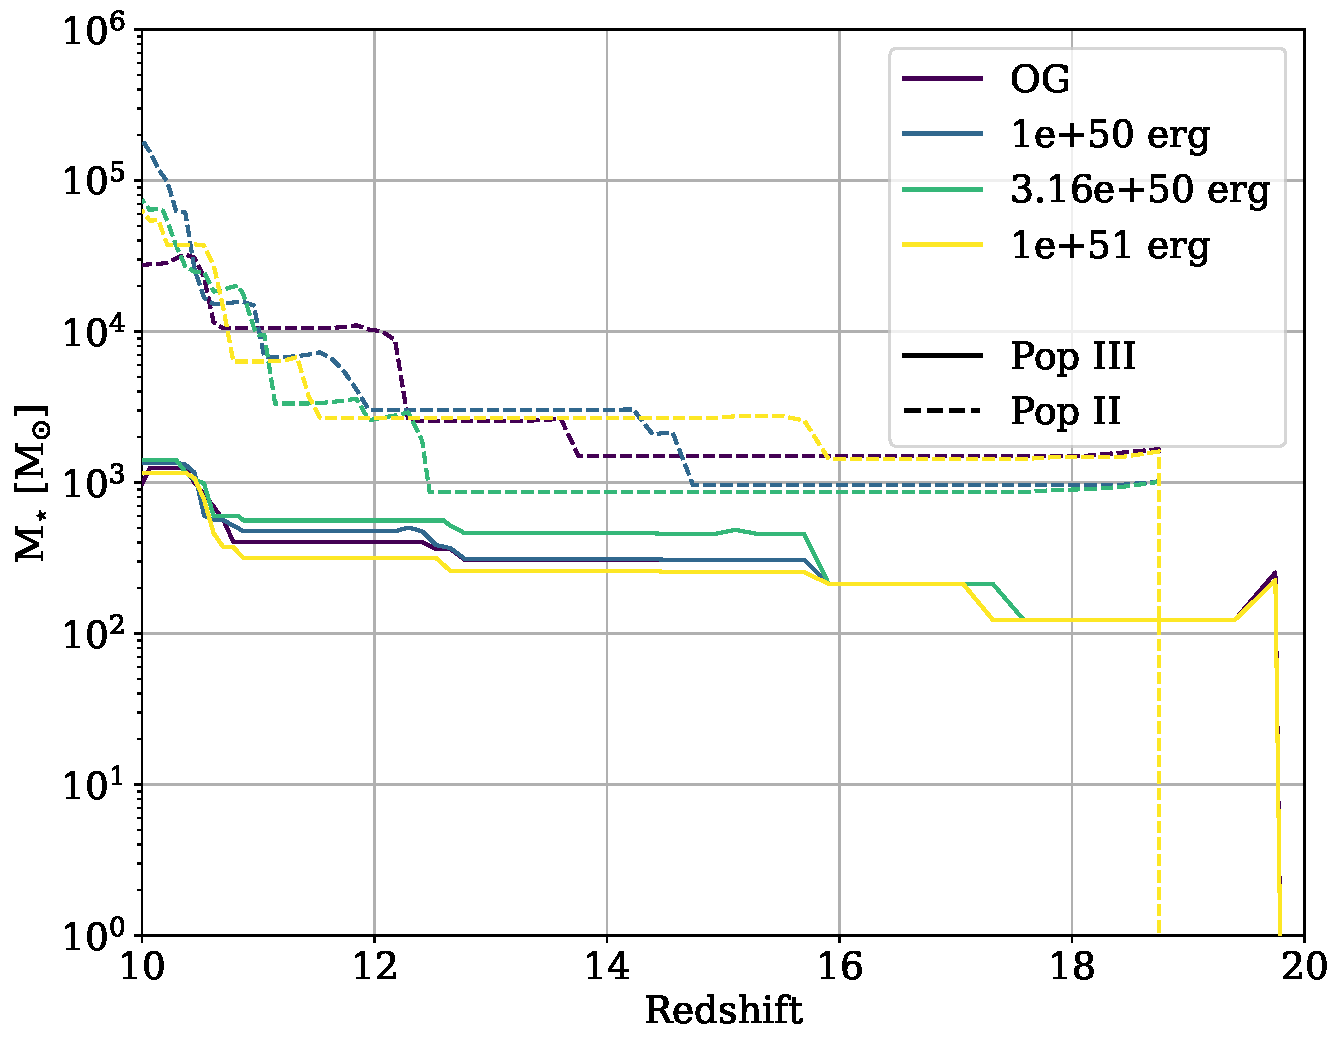
\includegraphics[width=0.4\textwidth]{plots/eng_stellar_mass.pdf} }}%
    \qquad
    \subfloat[\centering Delay Time Variation]{{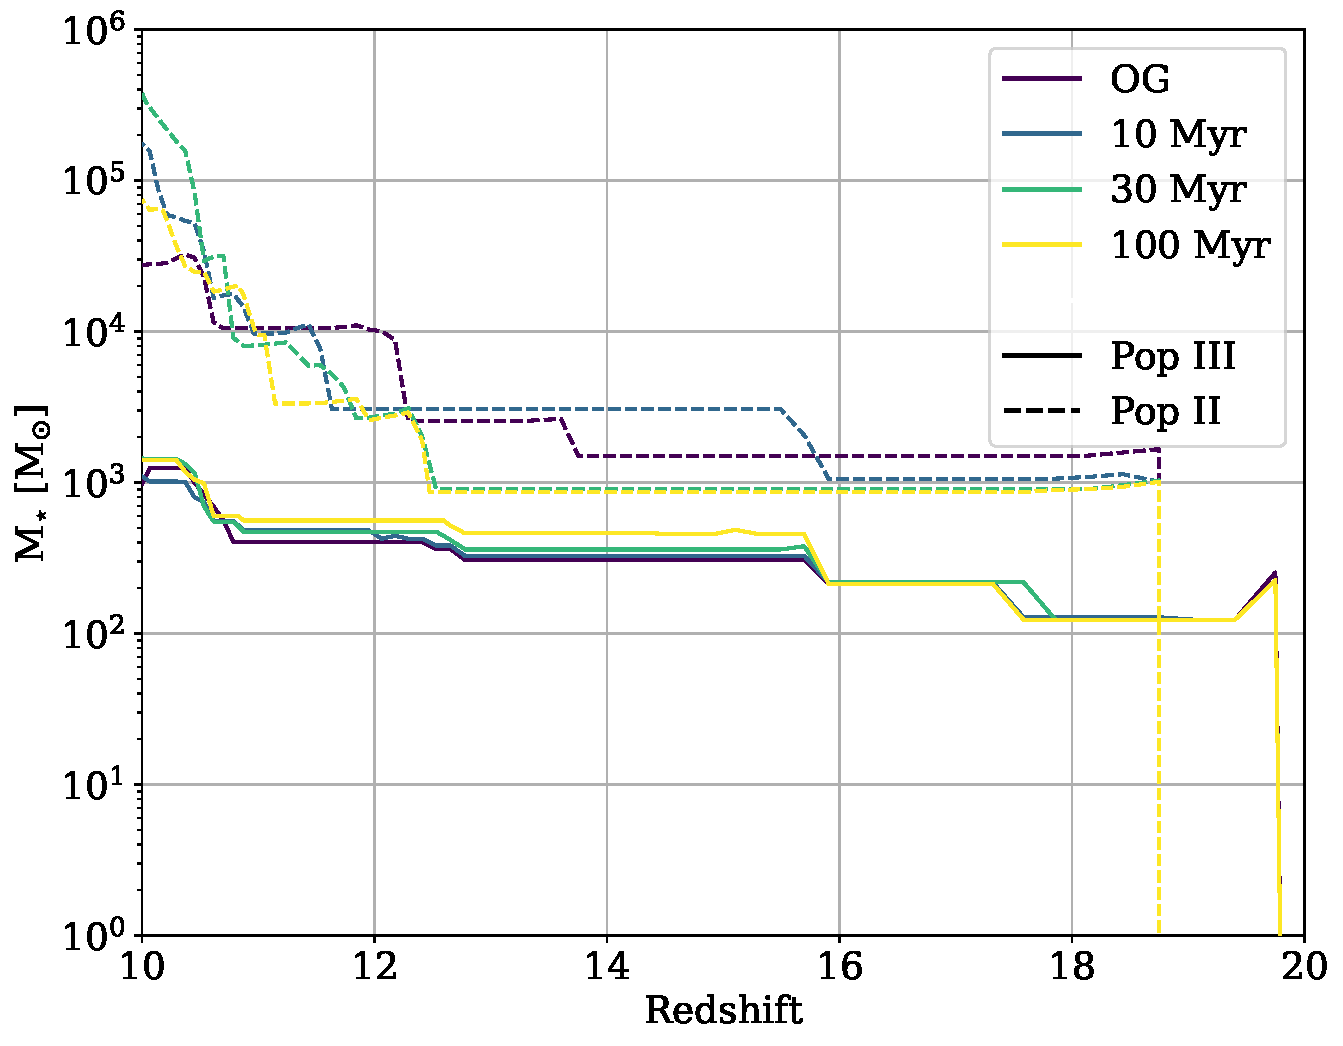
\includegraphics[width=0.4\textwidth]{plots/time_stellar_mass.pdf} }}%
    \caption{The total stellar mass of both Pop III and Pop II stars as a function of redshift. The solid lines are the total stellar masses of Pop III stars, and the dashed lines are total stellar masses of Pop II stars.}%
    \label{fig:ratio}%
\end{figure}

\begin{itemize}
    \item Riaz+22: compare with their Figure 1 and 3 (https://iopscience.iop.org/article/10.3847/2041-8213/ac8ea6/meta)
    \begin{itemize}
        \item Re. Figure 1: Looking at the redshift range between 10 and 20, and comparing with their halo masses between $10^7 - 10^9 M_\odot$ since this is the closest out halo gets to by the end of the simulation, we do see much higher stellar masses compared to them. For example, at z = 10, they see $10^3 - 10^5 M_\odot$ for Pop II stars and $10^1 - 10^2 M_\odot$ for Pop III stars. In our simulations at $z = 10$, we see a few$\times 10^4 M_\odot$ for Pop II stars, consistent with their results, and $\sim10^{3} M_{\odot}$ for Pop III stars, which is certainly larger than Riaz+22. However, they do give some generous ranges for the Pop II and Pop III stellar masses, so our results are not incompatible with Riaz+22.
        \item Re. Figure 3: This figure is very similar to the one from Yajima+23. We do see similar ratios overall (see Figure \ref{fig:ratio} above).
    \end{itemize}
    \item Yajima+23: compare with their Figure 4, third bullet point in their conclusion (https://arxiv.org/pdf/2211.12970.pdf)
    \begin{itemize}
        \item Re: Figure 4. I have made this same plot for our work. We have slightly lower values compared to Yajima. For all variation runs, for a stellar mass of $\sim10^{4.5} M_\odot$, we see a Pop III mass ratio of about $\sim10^{-1.5}$, as compared to Yajima's results of $\sim10^{-1}$. They have considerable scatter for their $z = 10$, 11, and 12 data. Certainly we see the same trend as them, as stellar mass increases, the ratio of Pop III stellar mass to total stellar mass decreases. We do see similar values at our maximum stellar mass value of $\sim10^{5.5} M_\odot$ having a mass ratio of $\sim10^{-2.25}$. An important thing to consider in this comparison is the much higher halo mass of their main halos. They look at a halo that grows to $5 \times 10^{11} M_\odot$ by $z = 9.5$, whereas our halo gets to $\sim2 \times 10^{8} M_\odot$ at $z = 10$ (see Figure \ref{fig:ratio} above).
        \item Based on these results, we certainly agree with their third bullet point. In general, the mass fraction of Pop III stars is less than 0.01 for halos with stellar masses $> 10^{4} M_\odot$ 
    \end{itemize}
\end{itemize}

We again thank the referee for the insightful review that helped
improve our paper.

\bibliographystyle{plainnat}
\bibliography{drenniks}

\end{document}